\section{Conceitos Gerais}\label{sec:concepts}
Este trabalho apresenta conceitos fundamentais relacionados ao desenvolvimento e funcionamento da extensão ESPEON (Engajamento e Supervisão do Processo de Ensino Online), uma ferramenta desenvolvida para navegadores Google Chrome com o objetivo de mensurar os níveis de atenção e engajamento de alunos em aulas remotas. A proposta da ESPEON é validar a efetividade da metodologia expositiva no contexto do ensino remoto, metodologia esta que, segundo Andreata (2019) \cite{ANDREATA2019}, baseia-se na transmissão de conteúdo por um orador, cabendo ao estudante uma postura predominantemente passiva de recepção e assimilação do conhecimento.

Para possibilitar o funcionamento da ESPEON, algumas tecnologias foram empregadas. Primeiro, o MongoDB - um banco de dados não relacional - orientado a documentos, amplamente utilizado no desenvolvimento de aplicações modernas, principalmente em ambientes que exigem escalabilidade, como os baseados em computação em nuvem. Esse banco de dados é gerenciado na nuvem por meio do serviço AtlasDB, oferecido pela MongoDB Inc., o qual simplifica a implantação, o gerenciamento e o escalonamento de instâncias MongoDB.

A comunicação entre a extensão e o MongoDB ocorre por meio de uma API (\textit{Application Programming Interface}), que define protocolos e regras para a interação entre sistemas, aplicativos ou serviços. Para este projeto, utiliza-se o framework Flask, escrito em Python, para a criação das APIs. Esse framework permite a criação ágil de aplicações web escaláveis e integráveis com diferentes bibliotecas. A arquitetura procedural da solução está disposta na Figura \ref{fig:figura1}.

\begin{figure}[ht]
\centering
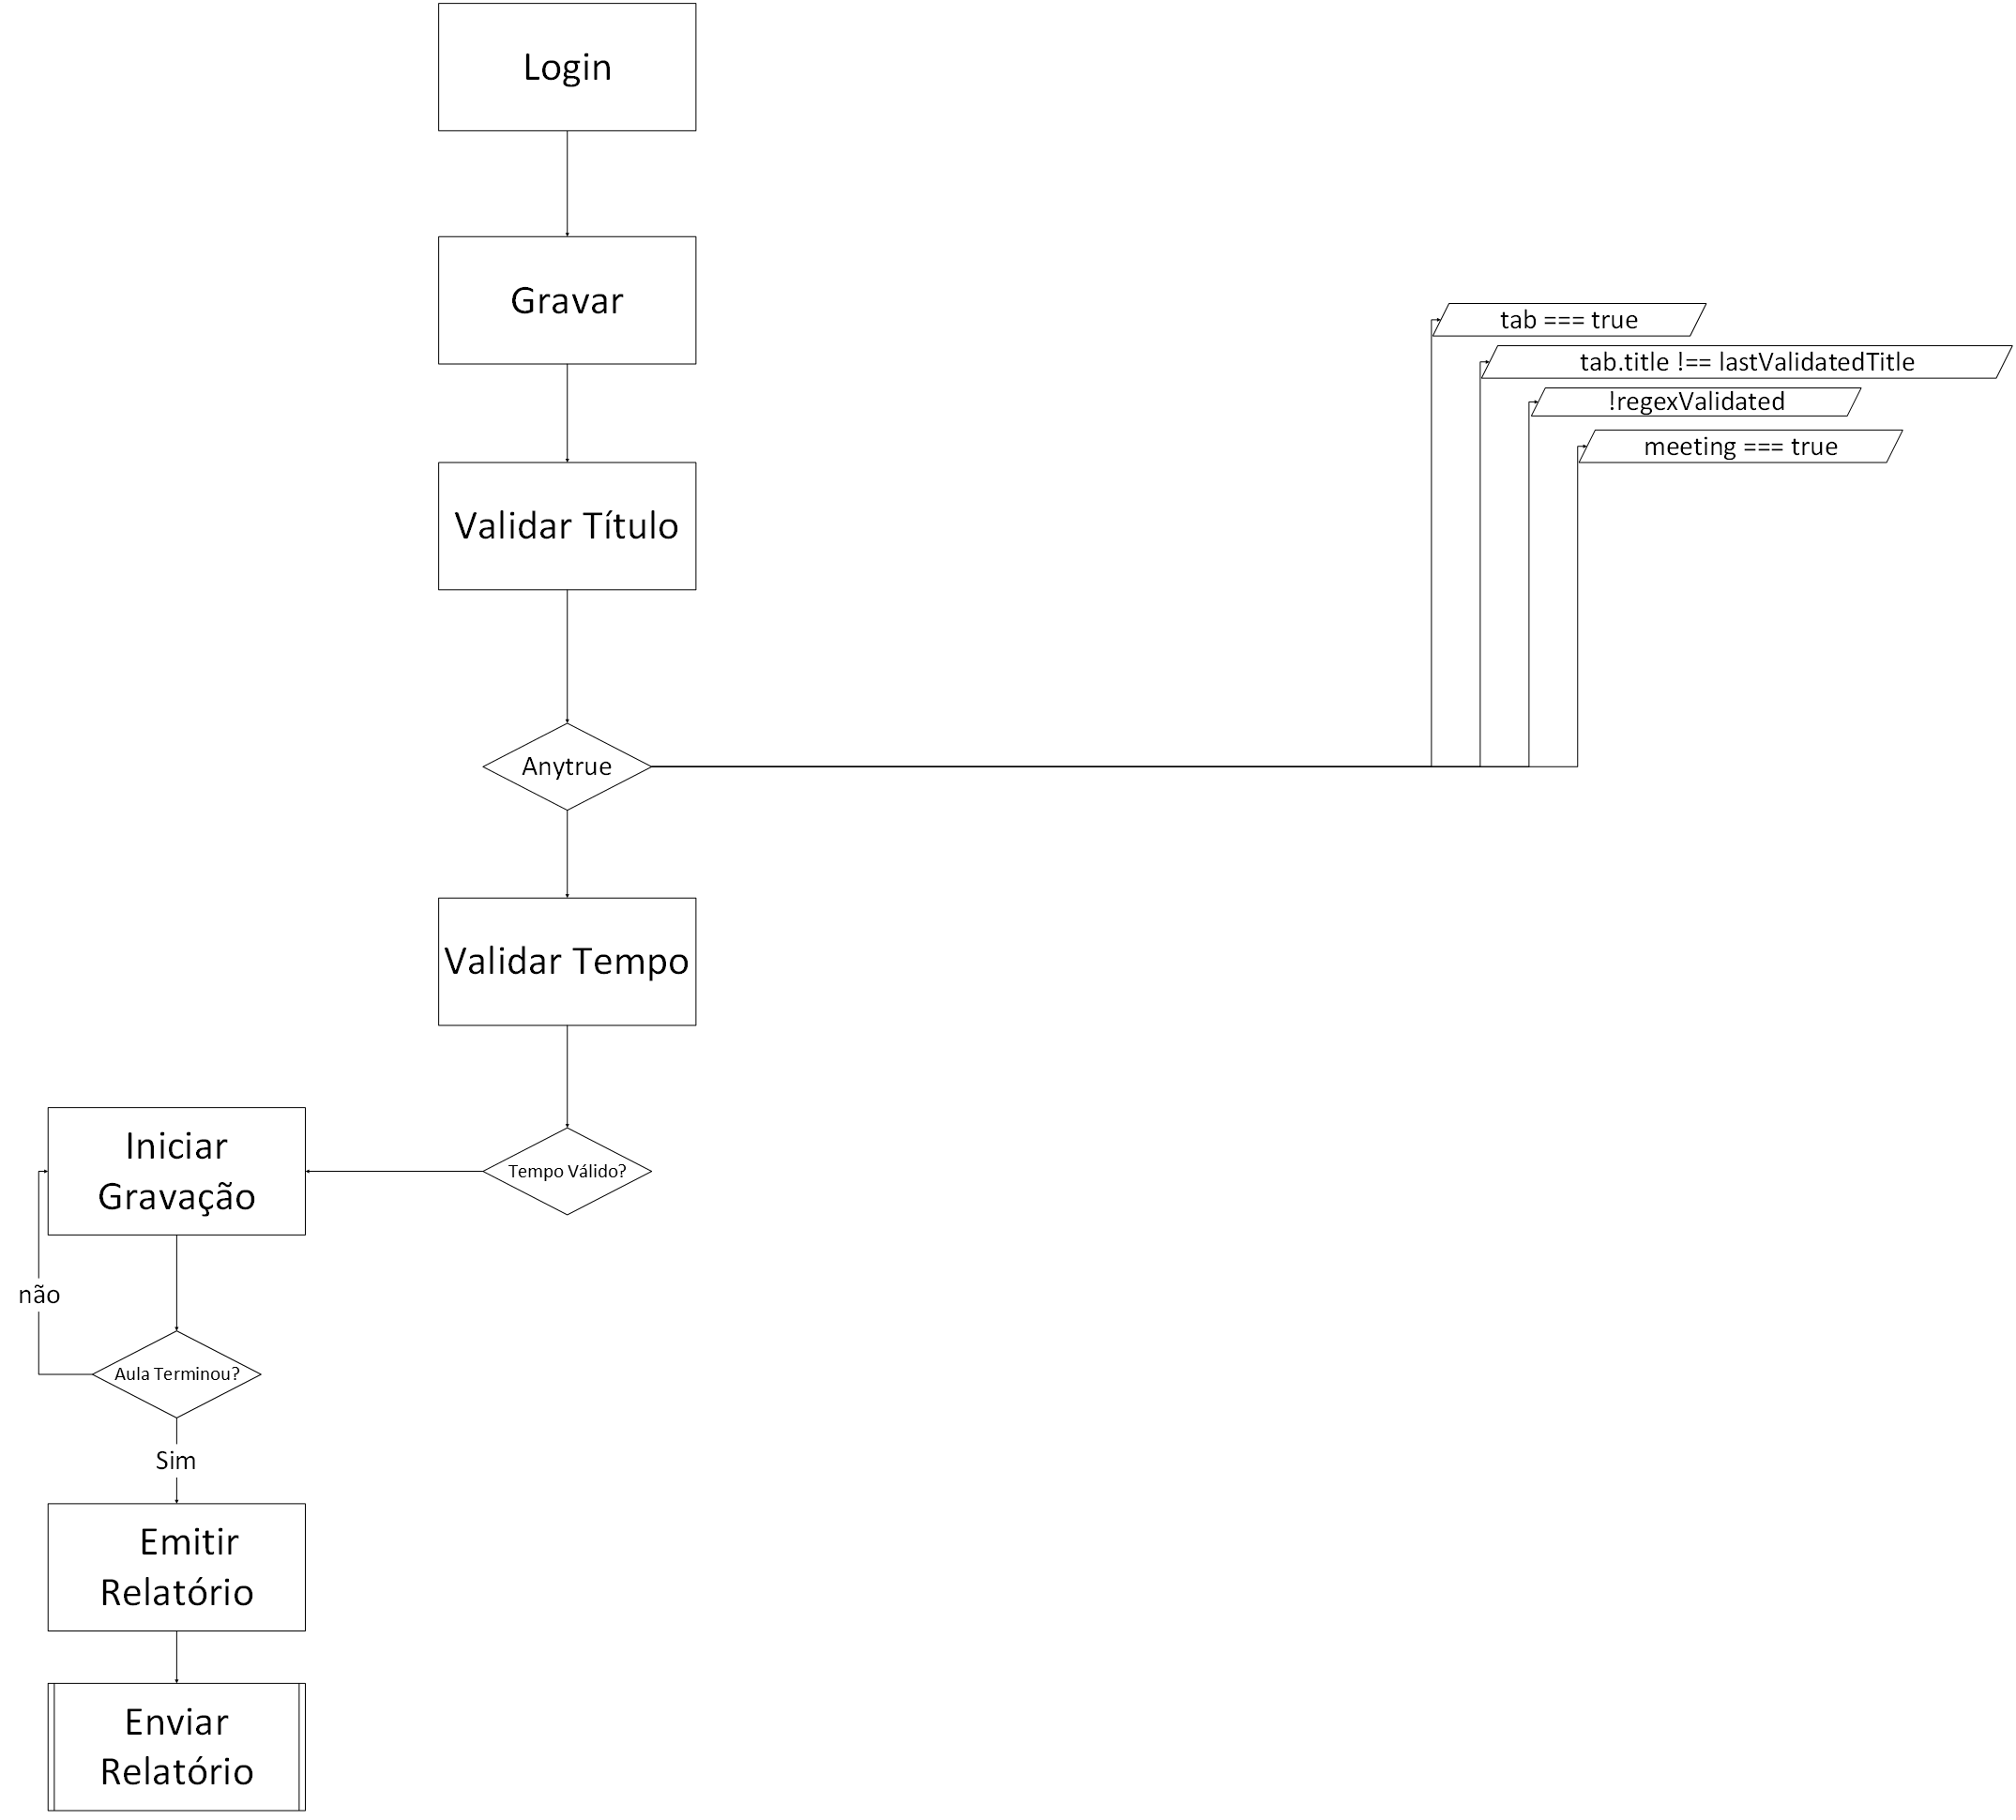
\includegraphics[width=.5\textwidth]{assets/images/arquitetura.png}
\caption{Arquitetura Conceitual}
\label{fig:figura1}
\end{figure}

Além disso, o processo de implantação da aplicação em ambiente de produção, o \textit{deploy}, ocorre, neste contexto, quando o banco de dados e a API são disponibilizados para acesso por inúmeros clientes. A operação e o comportamento da aplicação são constantemente monitorados por meio de \textit{logs}, que são registros estruturados de eventos e ações executadas pelo sistema. Por fim, vale destacar que a distribuição da extensão ocorre por meio da Chrome Web Store, a plataforma oficial do Google para disponibilização de extensões, aplicações e temas voltados ao navegador Chrome.